\subsection{Adapting movement initiation succeeding prediction errors: reinforcement learning}

\begin{figure}[h]
  \begin{flushleft}\textbf{A}\end{flushleft}
  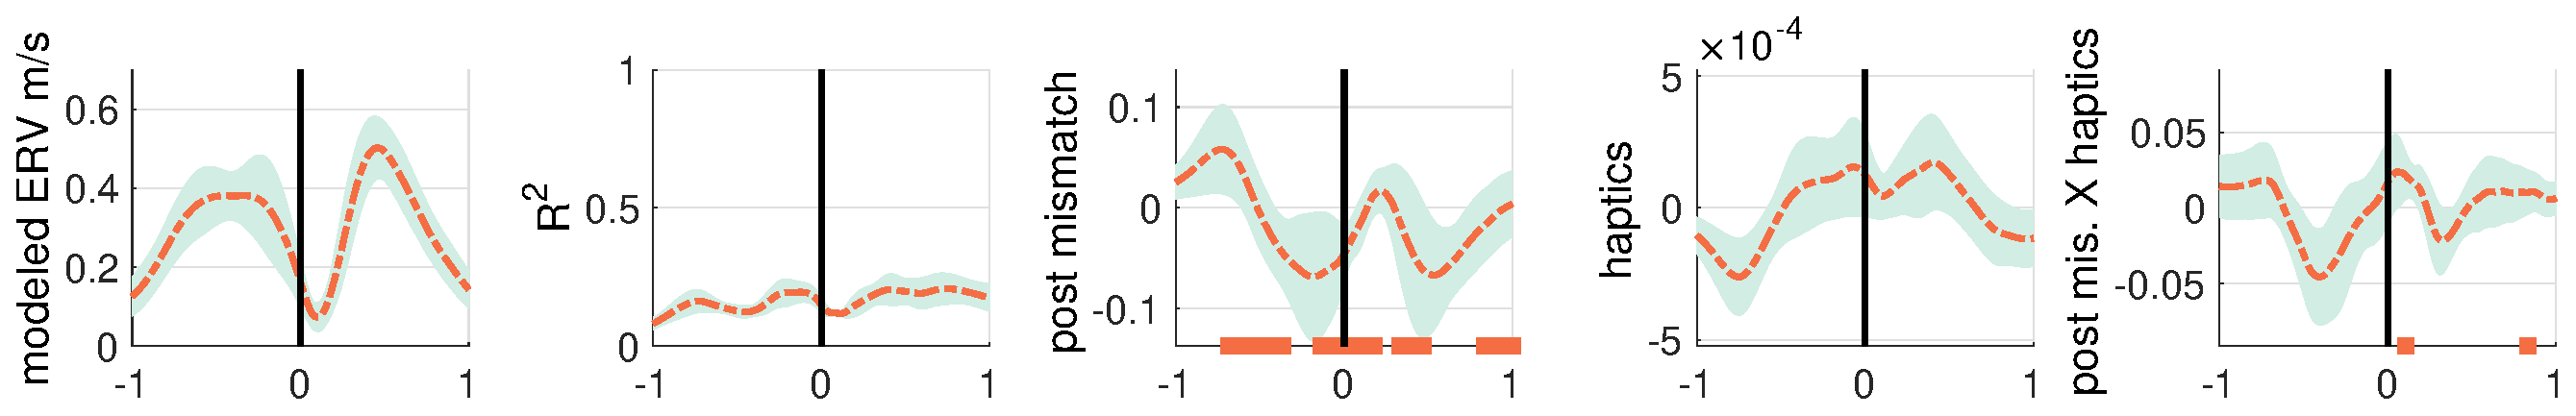
\includegraphics[width=\textwidth]{figures/vel_mocap_2.eps}
  \label{vel_erp_post_mismatch}
  \caption{Event-related velocity (ERV) succeeding premature collision.}
\end{figure}

-> run a model predicting subsequent behavioral adaptation (operationalized through rt? or acceleration?) including velocity at previous collision, whether there were haptics and the strength of PE signal (peak theta burst?)

% rendering the physics of the world impacting event processing and estimation of physics in the world